\documentclass[10pt, a5paper]{article}
\usepackage{pdfpages}
\usepackage{parallel}
\usepackage[T2A]{fontenc}
\usepackage{ucs}
\usepackage[utf8x]{inputenc}
\usepackage[polish,english,russian]{babel}
\usepackage{hyperref}
\usepackage{rotating}
\usepackage[inner=2cm,top=1.8cm,outer=2cm,bottom=2.3cm,nohead]{geometry}
\usepackage{listings}
\usepackage{graphicx}
\usepackage{wrapfig}
\usepackage{longtable}
\usepackage{indentfirst}
\usepackage{array}
\newcolumntype{P}[1]{>{\raggedright\arraybackslash}p{#1}}
\frenchspacing
\usepackage{fixltx2e} %text sub- and superscripts
\usepackage{icomma} % коскі ў матэматычным рэжыме
\PreloadUnicodePage{4}

\newcommand{\longpage}{\enlargethispage{\baselineskip}}
\newcommand{\shortpage}{\enlargethispage{-\baselineskip}}

\def\switchlang#1{\expandafter\csname switchlang#1\endcsname}
\def\switchlangbe{
\let\saverefname=\refname%
\def\refname{Літаратура}%
\def\figurename{Іл.}%
}
\def\switchlangen{
\let\saverefname=\refname%
\def\refname{References}%
\def\figurename{Fig.}%
}
\def\switchlangru{
\let\saverefname=\refname%
\let\savefigurename=\figurename%
\def\refname{Литература}%
\def\figurename{Рис.}%
}

\hyphenation{admi-ni-stra-tive}
\hyphenation{ex-pe-ri-ence}
\hyphenation{fle-xi-bi-li-ty}
\hyphenation{Py-thon}
\hyphenation{ma-the-ma-ti-cal}
\hyphenation{re-ported}
\hyphenation{imp-le-menta-tions}
\hyphenation{pro-vides}
\hyphenation{en-gi-neering}
\hyphenation{com-pa-ti-bi-li-ty}
\hyphenation{im-pos-sible}
\hyphenation{desk-top}
\hyphenation{elec-tro-nic}
\hyphenation{com-pa-ny}
\hyphenation{de-ve-lop-ment}
\hyphenation{de-ve-loping}
\hyphenation{de-ve-lop}
\hyphenation{da-ta-ba-se}
\hyphenation{plat-forms}
\hyphenation{or-ga-ni-za-tion}
\hyphenation{pro-gramming}
\hyphenation{in-stru-ments}
\hyphenation{Li-nux}
\hyphenation{sour-ce}
\hyphenation{en-vi-ron-ment}
\hyphenation{Te-le-pathy}
\hyphenation{Li-nux-ov-ka}
\hyphenation{Open-BSD}
\hyphenation{Free-BSD}
\hyphenation{men-ti-on-ed}
\hyphenation{app-li-ca-tion}

\def\progref!#1!{\texttt{#1}}
\renewcommand{\arraystretch}{2} %Іначай формулы ў матрыцы зліпаюцца з лініямі
\usepackage{array}

\def\interview #1 (#2), #3, #4, #5\par{

\section[#1, #3, #4]{#1 -- #3, #4}
\def\qname{LVEE}
\def\aname{#1}
\def\q ##1\par{{\noindent \bf \qname: ##1 }\par}
\def\a{{\noindent \bf \aname: } \def\qname{L}\def\aname{#2}}
}

\def\interview* #1 (#2), #3, #4, #5\par{

\section*{#1\\{\small\rm #3, #4. #5}}

\def\qname{LVEE}
\def\aname{#1}
\def\q ##1\par{{\noindent \bf \qname: ##1 }\par}
\def\a{{\noindent \bf \aname: } \def\qname{L}\def\aname{#2}}
}

\begin{document}
\title{Гибридные системы хранения данных\footnote{\url{alex_kls@mail.ru}, \url{https://lvee.org/en/abstracts/290}}}
\author{Александр Клыга, Minsk, Belarus}
\maketitle
\begin{abstract}
The concept of a hybrid data storage is covered. Main approaches to implement hybrid data storage systems are reviewed as well as modern development tendencies in FOSS.
\end{abstract}
В основе создания гибридных систем хранения данных лежит принцип объединения в  единое пространство хранения твердотельных и механических накопителей. В зависимости от подхода объединения дисков в массивы используется либо технология кэширования, при которой в медленным дискам добавляется кэш на быстрых флеш-дисках, либо реализуется архитектура многослойных СХД~\cite{Klyga-1}. Выбор конкретного подхода в реализации гибридных СХД определяется типом используемых накопителей, требуемыми параметрами быстродействия и надежности хранения данных. В большинстве решений программного-определяемых систем хранения данных, например, Ceph~\cite{Klyga-6}, Gluster~\cite{Klyga-7} используется оба подхода в реализации гибридных СХД. В файловых системах, например, таких как BtrFS~\cite{Klyga-5}, Bcachefs~\cite{Klyga-3} и ZFS~\cite{Klyga-4} предпочтение отдается технологиям кэширования данных. Однако, массовое развитие производства флеш-накопителей, активное использование нового интерфейса NVM Express~\cite{Klyga-2}, и возрастающие требования к доступности данных, меняют концепцию создания гибридных СХД.

Ключевой проблемой гибридной СХД является более высокое время отклика данных по сравнение с флеш-массивами (All-Flash Array, AFA), и не оптимальное использование возможностей флеш-накопителей с интерфейсом NVM Express, но при этом они обеспечивают более низкую цену хранения данных на механических накопителях (как правило, жесткие диски большой емкости с низкой скоростью вращения шпинделя).

Первым вариантом создания гибридных СХД с низким временем доступа к данным является использование многоуровневой~\cite{Klyga-1} схемы организации хранения данных, где на первом уровне располагаются AFA массивы хранения, а на втором и при необходимости на третьем уровне массивы хранения данных на механических накопителях (рисунок ниже).

\begin{center}
\begin{figure}[h!]
  \centering
  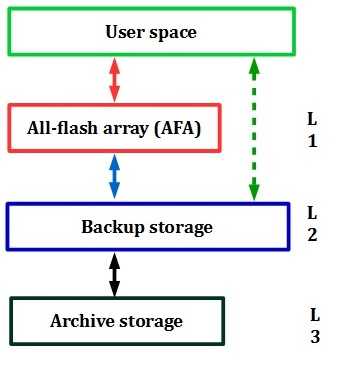
\includegraphics[width=7cm]{19_2018_Kliga1.jpg}
  %\caption{Конфигурация NFS v3}
  \label{Kliga1}
\end{figure}
\end{center} 
 

AFA-массивы на первом уровне (L1) при такой архитектурной реализации выступают в роли самостоятельных СХД, обеспечивающих высокую производительность для критически важных данных. По мере «остывания» данных они в режиме теневого копирования переносятся на второй уровень хранения на механических дисках с высокой скоростью вращения шпинделя. Удаление данных на первом уровне производится когда их показатель их востребовательности ниже установленного уровня определенного показателем «температуры данных», при этом при необходимости их резервная копия сохраняется на втором уровне хранения.

Данные со второго уровня хранения (L2) так же по мере «остывания» теневым копированием переносятся на третий архивный уровень (L3) на котором используются механические накопители большой емкости, но с низкой скоростью вращения шпинделя. Для хранения данных с некритичным временем доступа, в пользовательском пространстве создается точка монтирования на второй уровень (L2) СХД. Управление размещением данных на уровнях и организацией доступа к ним осуществляется с помощью контроллера SDS (software-defined storage), например, на базе решения openSDS~\cite{Klyga-8}.

Основные преимущества данного варианта создания гибридной СХД:

\begin{itemize}
  \item возможность обеспечения хранения данных с учетом требований к критичности времени доступа к данным;
  \item на каждом уровне отдельное хранилище данных может использоваться как самостоятельно устройства с функцией централизованного управления и возможностями резервного хранения данных;
  \item использование функционала теневого копирования для резервирования данных между отдельными хранилищами или уровнями;
  \item единый центр управления хранением данных на базе решений FOSS.
\end{itemize}

Основные недостатки:

\begin{itemize}
  \item невозможность использования технологии тиринга между уровнями хранения данных;
  \item высокая нагрузка на внутреннюю шину подключения хранилищ данных между уровнями из-за операций теневого копирования;
  \item сложность создания архитектуры и настройки под заданные параметры производительности.
\end{itemize}

Вторым вариантом реализации гибридного СХД с низким временем доступа  является использование возможностей накопителей с интерфейсом NVM Express, с двухуровневой схемой структурной схемой СХД с использованием технологии тиринга на первом уровне хранилища данных в массивах AFA (рисунок ниже). В основе этого варианта лежит концепция использования накопителей с интерфейсом  NVM Express в качестве элементов хранения данных RAM пользователя, и основным хранилищем данных на AFA-массивах.  Между двумя слоями в AFA первого уровня (L1) используется технология тиринга, когда «теплые данные из первого слоя переносятся во второй слой. Если же места для хранения данных исчерпано, либо данные стали <<остывшими>> они переносятся на второй уровень хранения (L2).

Этот вариант реализации гибридной СХД позволяет оптимально использовать возможности всех типов флеш-накопителей, а при необходимости возможности по хранению данных могут расширены за счет добавления новых уровней.

\begin{center}
\begin{figure}[h!]
  \centering
  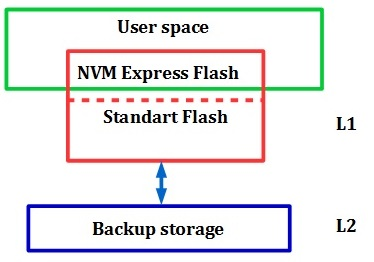
\includegraphics[width=7cm]{19_2018_Kliga2.jpg}
  %\caption{Конфигурация NFS v3}
  \label{Kliga2}
\end{figure}
\end{center} 

Основные преимущества данного варианта создания гибридной СХД:

\begin{itemize}
  \item возможность обеспечения высокой доступности данных;
  \item более простая схема реализации хранилища данных;
  \item использование функционала технологии тиринга и теневого копирования для резервирования данных между отдельными уровнями;
  \item высокая доступность данных для пользователя.
\end{itemize}

\begin{thebibliography}{20}
\bibitem{Klyga-1} Многослойные и многоуровненые системы хранения данных // LVEE 2017. \url{https://lvee.org/ru/abstracts/238}
\bibitem{Klyga-2} NVM Express: the official site. \url{http://www.nvmexpress.org/}
\bibitem{Klyga-3} Bcachefs: An advanced new filesystem for Linux. \url{https://bcachefs.org}
\bibitem{Klyga-4} ZFS: Zettabyte File System (OpenZFS project). \url{https://open-zfs.org}
\bibitem{Klyga-5} Btrfs: Btrfs is a modern CoW filesystem for Linux: // btrfs official site. \url{https://btrfs.wiki.kernel.org/index.php/Main\_Page}
\bibitem{Klyga-6} Ceph: The future of storage. \url{https://ceph.com/}
\bibitem{Klyga-7} Gluster: Storage for your Cloud. \url{https://gluster.org}
\bibitem{Klyga-8} OpenSDS Project. \url{https://www.opensds.io/}
\end{thebibliography}
\end{document}
